\section{Вступ}

Доставка вантажів автотранспортом є важливим етапом серед процесів дистрибуції. Особливо важливою частиною цього процесу є фінальна доставка до дверей клієнта, відома як «остання миля». Дослідження показують що саме цей етап є одним з найдорожчих та найскладніших у організації. Саме тому багато сучасних розробок зосереджено на оптимізації, покращені та спрощенні цього процесу.

Так наприклад була розроблена система оптимізації маршрутів транспортних засобів, що дозволяє скоротити витрати на доставку за рахунок кращого планування маршрутів кожного транспортного засобу, що дозволяє обслужити більше точок доставки за раз, а значить і скоротити загальну кількість необхідних автомобілів \cite{art1}. Цей результат є дуже важливим не лише з економічних, а й з екологічних причин, оскільки зменшення кількості транспортних засобів, що використовується, означає також і зменшення кількості шкідливих викидів у атмосферу.

На жаль при впровадженні систем оптимізації маршрутів транспортних засобів виринає багато проблем, пов’язаних з тим, що під час виконання доставки завжди відбуваються ті чи інші відхилення від плану, яким би оптимальним він не був. Подібні відхилення в кожному випадку потребують коригування плану через комунікацію з диспетчером.

Практика показує що водії-експедитори та кур'єри скоріше починають виконувати доставки поза планом, якщо процес комунікації з диспетчером та коригування планів недостатньо простий та ефективний. Наприклад необхідність дзвонити диспетчеру кожен раз або використовувати програму фіксації позапланових ситуацій на смартфоні з сенсорним управлінням затримує водія та відволікає від основної задачі управління транспортним засобом.

В сучасних бортових системах автомобілю все частіше з'являється елементи керування голосом \cite{art2,Kravchenko_2009,Heisterkamp_2001}. Крім того використання голосового інтерфейсу дозволить звільнити руки водія та полегшити збір додаткової статистичної інформації, що полегшить та покращить планування наступних маршрутів \cite{conf9}. На жаль найкращі сучасні системи розпізнавання голосу не можуть бути встановлені на мобільний пристрій і працюють тільки в у онлайн режимі. Але для задачі дистрибуції може бути важко забезпечити постійний доступ до мережі інтернет, оскільки доставка може відбуватися до місць/регіонів, де навіть мобільний GPRS інтернет відсутній, або має надто низьку швидкість передачі даних для роботи зі звуком. Тому актуальним залишається запит подальшого вдосконалення автоматизації голосової взаємодії для підвищення ефективності системи дистрибуції.

\section{Аналіз літературних даних та постановка проблеми}

Японський дослідник з університету Осаки Ішігуро Хіроші з колегами вивчали різні аспекти комунікації та інформаційно-комунікаційних технологій, як, наприклад, використання комунікації з людиноподібними роботами в якості терапевтичної дії для людей похилого віку \cite{Nishio_2015}, аутистів \cite{Kumazaki_2016} чи просто замкнутих у собі людей, педагогічної дії щодо дітей та немовлят \cite{Park_2015} тощо. Зокрема він проводив дослідження голосової комунікації двох людей опосередковано через комп’ютер \cite{Ishiguro_2016}.

У цьому дослідженні пара спілкувалася на загальні теми, обираючи варіанти своєї репліки із заздалегідь написаного дерева варіантів, свого роду сценарію. Жодному з партнерів не потрібно було нічого промовляти вголос: людині надавався набір з варіантів реплік на вибір, потрібно було лише натиснути на ту з них, яку б вона хотіла  промовити, і ця репліка лунала з динаміків. У залежності від використаної репліки програма вибирала з дерева сценаріїв можливі варіанти відповідей і надавала їх на вибір співрозмовнику. Співрозмовник у свою чергу, чуючи репліку першої людини, обирав свою з поданих варіантів. Це дослідження було спрямоване на подолання сором’язливості при спілкуванні з особами протилежної статі (що є особливо актуальним для Японії). Але такий підхід заздалегідь написаного дерева сценаріїв комунікації можна використовувати і в інших сферах.

У доповіді на світовому психологічному конгресі 2016 проф. Ішігуро демонстрував використання цього сценарного підходу для роботів на виставках та в музеях. Що б уникнути необхідності розпізнавання голосу в шумному середовищі, поряд з експонатом ставиться людиноподібний робот та монітор, на якому показані варіанти запитань. Натискаючи на різні репліки, відвідувач може спілкуватися з роботом по заздалегідь написаному дереву сценаріїв, розпитуючи його про експонат, а робот буде відповідати голосом.

На жаль для управління дистрибуцією постає зворотне завдання — водій має повідомити певну інформацію в систему і при цьому не повинен відволікатися на натискання кнопок на екрані. Тому пряме використання такої технології неможливе. Але застосування підходу описання всіх можливих сценаріїв комунікації в залежності від контексту дозволить знизити кількість інформації, яку треба розпізнати, а отже і підвищити якість \cite{art2}.

Сучасні системи розпізнавання мови в більшій своїй частині засновані на статистичних методах, використовують потужний апарат теорії ймовірностей та математичної статистики, що дає змогу суттєво підвищити якість розпізнавання. Основні методи розпізнавання мови — це приховані Марківські моделі та штучні нейронні мережі \cite{Makovkin_2006, Gefke_2012}. Але у сучасних системах більш поширеними є моделі на нейронних мережах, оскільки вони мають більшу швидкодію та стійкість до шумів \cite{Hinton_2012}.

Традиційним підходом до вирішення проблеми є розпізнавання голосової команди і перетворення її на текстову. Існує досить багато таких систем і вони доволі якісно виконують свою задачу. Але для якісного розпізнавання довільного голосового сигналу у текст, модель повинна бути достатньо велика, включно з великими контекстно-залежними словниками. Саме з цієї причини кращі сучасні системи розпізнавання мови як то Google Voice Search не можуть бути встановлені на мобільний пристрій і працюють тільки в у онлайн режимі. На жаль для задачі дистрибуції може бути важко забезпечити постійний доступ до мережі інтернет, оскільки доставка може відбуватися до місць/регіонів, де навіть мобільний GPRS інтернет відсутній, або має занадто низьку швидкість передачі даних для роботи зі звуком.

Наразі існує новий підхід до голосового управління, заснований на теорії несилової взаємодії \cite{Teslia_2010} — рефлекторна система голосового управління \cite{Egorchenkov_2016}. Ідея, покладена в основу цього підходу, полягає в тому, щоб замість переведення голосової інформації в текстову репрезентацію, аналізувати безпосередньо інформаційну складову сказаного, визначаючи, яку з відомих реакцій потрібно виконати. «Традиційні системи розпізнавання мови засновані на принципі: „усна мова“ → „репрезентація мови набором лінгвістичних конструкцій“ → „розуміння мови“. На основі теорії несиловой взаємодій може бути запропонована інша модель розпізнавання природної мови: „усна мова“ → „розрахунок несилової (інформаційної) взаємодії на реакції“ → „реакція (розуміння чи поведінка)“» \cite{Teslia_2014}.

Така модель розпізнавання називається рефлекторною, оскільки побудована за аналогією зі структурою умовного рефлексу, в якому виділяються афектори, центральний компонент та ефектори. Така модель може бути добре поєднана з ідеєю використання дерева сценаріїв, оскільки сценарії також складаються із реакцій, і одиницею моделювання стає не лінгвістична особливість мовлення, а реакція (або команда), яка може бути врахована автоматизованою системою розрахунку маршрутів. Тобто, суть цього підходу полягає в тому, щоб перейти до іншої одиниці розпізнавання мови. У психології дискурсивного мислення і рефлексивній психології також накопичено досвід аналізу мови, через виокремлення інших одиниць — функціональних висловлювань \cite{Naydonov_2008}.

Оскільки в такій системі не потрібні словники, складні інтелектуальні моделі аналізу тексту та граматики, вони мають низку переваг порівняно з традиційними системами: багатодикторність, варіабельність природної мови, можливість обробки команд офлайн прямо на пристрої, робота в умовах шумів (неконтрольованого акустично середовища), простота алгоритмів та менша складність і ціна реалізації \cite{Teslia_2013}.

Проблема полягає в тому, що існуючі способи автоматизації голосової взаємодії не можуть забезпечити задач дистрибуції через суперечність між умовами такої діяльності і необхідною потужністю приладів для розпізнавання голосового сигналу в текстовий, що використовується в більшості існуючих моделей. Ідея полягає в тому, що розроблення моделі голосової взаємодії без блоку переведення звуку голосу в текст може принципово покращити автоматизацію голосової взаємодії в системах контроля дистрибуції.

Висунуто гіпотезу що поєднання двох найбільш перспективних напрями, виявлених у результаті аналізу, дає змогу запропонувати нове принципове рішення і побудувати рефлекторну модель голосової взаємодії в задачах управління дистрибуцією.

\section{Мета та задачі дослідження}
Метою дослідження є підвищення ефективності та зручності роботи водіїв в системах дистрибуції за рахунок розробки та використання інтелектуальних рефлекторних систем голосової взаємодії без блоку переведення звуку голосу в текст, що дасть змогу автоматизувати певні процеси управління дистрибуцією, покращуючи рівень сервісу та знижуючи витрати.

Задача полягає в тому, щоб за рахунок створення контекстної моделі голосової взаємодії в системах диспетчерського контролю за рухом автотранспорту адаптувати використання інтелектуальних рефлекторних систем голосового управління до задач дистрибуції, та порівняти ефективність різних варіантів реалізації таких систем.


\section{Матеріали та методи досліджень}

\subsection{Дерево сценаріїв як метод представлення змісту і контекстів голосової взаємодії}

В основу контекстної моделі голосової взаємодії покладено логічні сценарії взаємодії на тему управління дистрибуцією, які мають враховувати параметри основних причин невідповідності реальної ситуації запланованому маршруту, наприклад, запізнення або відмови обслуговування на точці доставки тощо \cite{art3}. Це дає змогу отримати інформацію для прийняття рішення про повернення вантажу на склад, про відміну чи відкладення обслуговування однієї точки доставки, щоб мати можливість встигнути на іншу, більш важливу, про зміну маршруту для об’їзду затору або про утворення нового маршруту з резервною машиною тощо.

Для представлення дерева сценаріїв найкраще підходить орієнтований граф, в якому вершини позначають стан системи (контексти) та діалогові фрази, які буде озвучувати система, а ребра — зміст реплік водія (стимули), які можуть бути сприйняті системою в кожній конкретній вершині. Реакція на стимул може привести до переходу між станами, отже орієнтоване ребро проводиться від тієї вершини в якій стимул може бути сприйнятий, до тієї, в який стан система перейде в якості реакції на стимул. Отже множина всіх ребер, що виходять з вершини, позначають перелік стимулів, між якими треба проводити розпізнавання для стану, що відповідає цей вершині.

Кожна вершина графу позначає контекст системи який обмежує можливі репліки які система може сприйняти в цьому стані. Такий підхід дозволяє суттєво підвищити якість розпізнавання за рахунок зменшення кількості можливих реакцій. До того ж це дозволяє скоротити команди, оскільки пропадає вимога їх глобальної унікальності. Однаковий контекст може бути одночасно в декількох вершинах, якщо ці вершини мають однаковий набір ребер що з них виходять.

\subsection{Метод інтелектуальних рефлекторних систем для побудови рефлекторної системи голосового управління}

Для побудови системи формалізації голосової взаємодії був використаний метод інтелектуальних рефлекторних систем. Він створений на основі теорії несилової взаємодії - комп'ютерній моделі світу, в якій фізичний рух описаний як стохастичні переміщення зі швидкістю світла на субатомному рівні. Формули виведені з такої моделі руху були використані для опису взаємодії довільних об'єктів а також для моделювання статистичних закономірностей у тексті \cite{Teslia_2010}.

Для побудови інтелектуальних рефлекторних систем припускається залежність сумісної умовної ймовірності реакції від безумовної ймовірності реакції та часткових умовних ймовірностей реакції в цій системі підкоряється законам збереження імпульсу в комп'ютерній моделі, і можуть бути розраховані по відповідним формулам.

Алгоритмічної основою таких систем є рефлекторний метод обчислення адекватної реакції на сукупність різних слабоструктурованих вхідних впливів.

Схема реалізації цього методу включає етапи:

1. Розрахунок визначеності для інтелектуальної системи відносно всіх вхідних впливів і можливих реакцій.

Аналогія визначеності реакцій і впливів в комп'ютерній моделі світу --- це імпульс матеріальних об'єктів. У такій моделі розглядаються дві групи об'єктів --- що впливають шляхом «зіткнення» та передачі власної інформації (імпульсу) об'єктам, на які здійснюється вплив (відповідно можливим реакціям):

\[
d(A_i)=\pm0.5\sqrt{\frac{p(A_i)}{1-p(A_i)}+\frac{1-p(A_i)}{p(A_i)}-2};
\]

\[
i(A_i)=\sqrt{d^2(A_i)+1};
\]

\[
d(A_i/B_j)=\pm0.5\sqrt{\frac{p(A_i/B_j)}{1-p(A_i/B_j)}+\frac{1-p(A_i/B_j)}{p(A_i/B_j)}-2};
\]

\[
i(A_i/B_j)=\sqrt{d^2(A_i/B_j)+1},
\]

\noindent
де: $p(A_i)$ --- безумовна ймовірність вибору реакції $A_i$; $d(A_i)$ --- визначеність щодо реакції $A_i$; $i(A_i)$ --- інформованість щодо реакції $A_i$; $p(A_i/B_j)$ --- умовна ймовірність вибору реакції $A_i$ (при існуванні впливу $B_j$); $d(A_i/B_j)$ --- визначеність щодо реакції $A_i$ при умові впливу $B_j$; $i(A_i/B_j)$ --- інформованість щодо реакції $A_i$ при умові впливу $B_j$.

2. З інформаційно-ймовірнісної інтерпретації формули релятивістського додавання швидкостей отримано додаткову визначеність, що є у впливаючих об'єктів відносно реакцій (швидкість руху впливаючих об'єктів відносно об'єктів, на які здійснюється вплив):

\[
\Delta d(A_i/B_j)=d(A_i/B_j)\cdot i(A_i)-d(A_i)\cdot i(A_i/B_j)
\]

\noindent
де $\Delta d(A_i/B_j)$ --- додаткова визначеність щодо реакції $A_i$ яку надає вплив $B_j$.

3. З інформаційно-ймовірнісної інтерпретації закону збереження імпульсу (\ref{eq:tnv11}) розраховано сумарний вплив на реакцію інтелектуальної системи. Аналог «удару» безлічі рухомих об'єктів (відповідних дій) в об'єкти, відповідні реакцій

\[
d_\Sigma(A_i) = \sum_j \Delta d(A_i/B_j); \\
\]

\[
i_\Sigma(A_i) = \sqrt{\Delta d^2(A_i/B_j)+1},
\]

\noindent
де $d_\Sigma(A_i)$ --- сумарна додаткова визначеність щодо реакції $A_i$ під впливом всіх подій $B_j$; $i_\Sigma(A_i)$ --- сумарна доповнювальна інформованість щодо реакції $A_i$ під впливом усіх подій $B_j$.

4. Обчислюється нова визначеність реакцій (аналог нової швидкості руху після отриманого під час зіткнення з впливаючими об'єктами імпульсу)

\begin{equation}
\label{eq:ifron2}
d(A_i/B)=d_\Sigma(A_i)\cdot i(A_i)+d(A_i)\cdot i_\Sigma(A_i),
\end{equation}


\[
i(A_i/B) = \sqrt{d^2(A_i/B)+1},
\]

\noindent
де $d(A_i/B)$ --- нова визначеність щодо реакції $A_i$ з урахуванням впливу всіх подій $B_j \in B$; $i(A_i/B)$ --- нова інформованість щодо реакції $A_i$ з урахуванням впливу всіх подій $B_j \in B$.

5. За необхідності з можна обчислити сумісну умовну ймовірність реакції $A_i$ (при існуванні всіх впливів $B_j \in B$)

\[
p(A_i/B)=0.5+\frac{d(A_i/B)}{2i(A_i/B)};
\]

\noindent
де $p(A_i/B)$ --- сумісна умовна ймовірність реакції $A_i$ (при існуванні всіх впливів $B_j \in B$).

Для формалізації голосової інформації використано систему з двох основних модулів: автоматичного фонетичного стенографа і ядра рефлекторної системи голосового управління (РСГУ), поточна реалізація яких визначає умови їх використання в моделі голосової взаємодії водія при диспетчерському контролі за рухом автотранспорту (рис. \ref{img:rsgu_struct}).

\begin{figure}[htb]
	\centering
	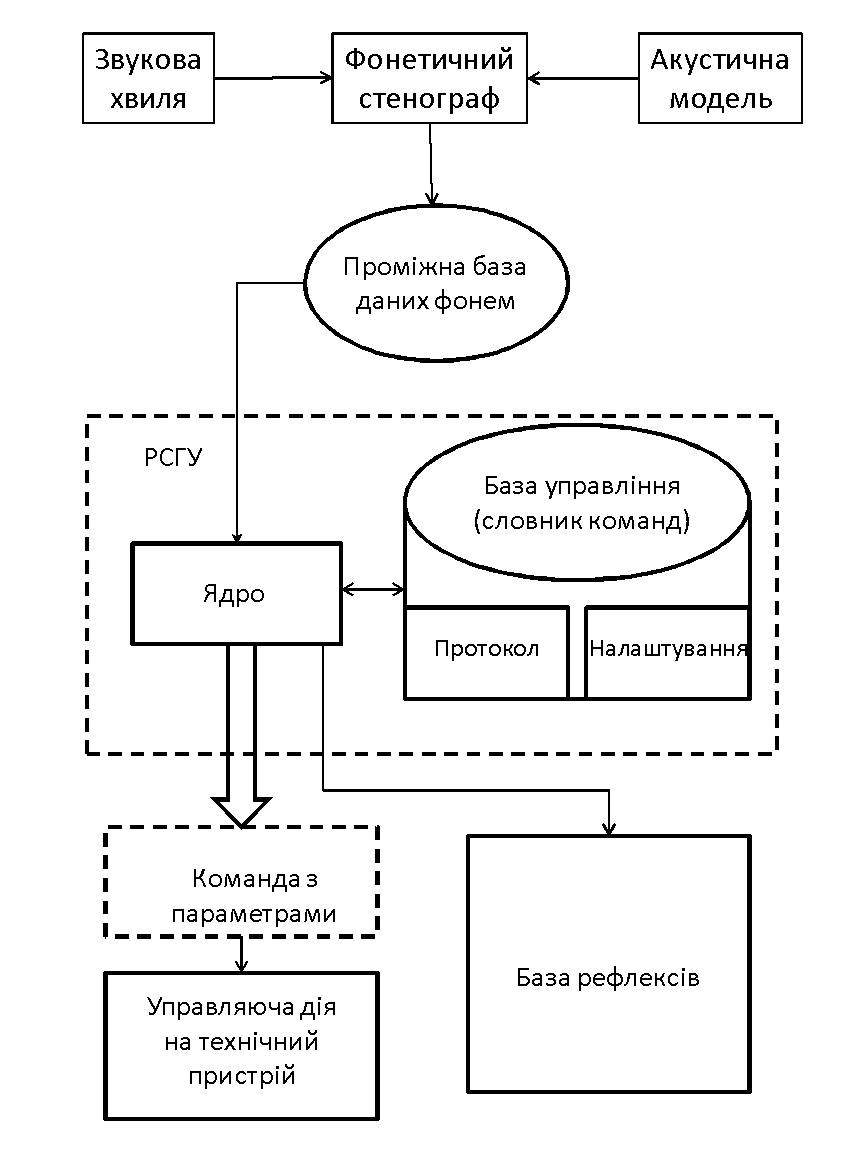
\includegraphics [width=.5\linewidth] {rsgu_struct}
	\caption{Структура системи формалізації голосової інформації в моделі голосової взаємодії водія при диспетчерському контролі за рухом автотранспорту}
	\label{img:rsgu_struct}
\end{figure}

Застосування алгоритму фонетичного стенографа дозволяє будувати послідовність контекстів для мовного сигналу без використання будь-якого словника. Для цієї мети будується деяка генеративна граматика, яка може синтезувати всі можливі модельні сигнали безперервної мови для будь-якої послідовності фонем. В рамках побудованої моделі будується алгоритм пофонемного розпізнавання для невідомого сигналу з використанням контекстів та можливих реакцій на них.

У розглянутій системі формалізації голосової інформації (рис. \ref{img:rsgu_struct}) вхідною інформацією виступає голосова команда, яка може бути представлена звуковою хвилею; вихідною ж інформацією буде виступати процес керуючого впливу на об’єкт управління, тобто відбуватиметься виконання розпізнаної команди відповідно до попередньо заданих голосом параметрам.

Сама система формалізації голосової інформації в процесі роботи буде генерувати потрібні візуальні і голосові інформаційні повідомлення водію, це, в свою чергу, надає можливість відслідковувати процес розпізнавання команд, реакції на них і, крім того, дозволяє в реальному масштабі часу змінювати поведінку системи в разі потреби.

\section{Результати класифікації голосових команд в системах управління дистрибуцією}

\subsection{Опис розробленої контекстної моделі голосової взаємодії в системах диспетчерського контролю за рухом автотранспорту}

Для створення контекстної моделі голосової взаємодії в системах диспетчерського контролю за рухом автотранспорту були зібрані статистичні дані, зауваження та коментарі щодо процесу доставки різних вантажів автомобільним транспортом у провідних логістичних компаніях. Систематизувавши та обробивши зібрані оригінальні коментарі до статусу доставки, що використовуються в різних компаніях, розроблено дерево сценаріїв для суб’єктів дистрибуції «склад – дорога – точка доставки» \cite{art3}.

Повне дерево сценаріїв усіх етапів дистрибуції «склад – дорога – точка доставки» в контекстній моделі голосової взаємодії водія в системі диспетчерського контролю за рухом автотранспорту наведено на рис. \ref{img:13_complete_scenario_graph}.

\begin{figure}
	\centering
	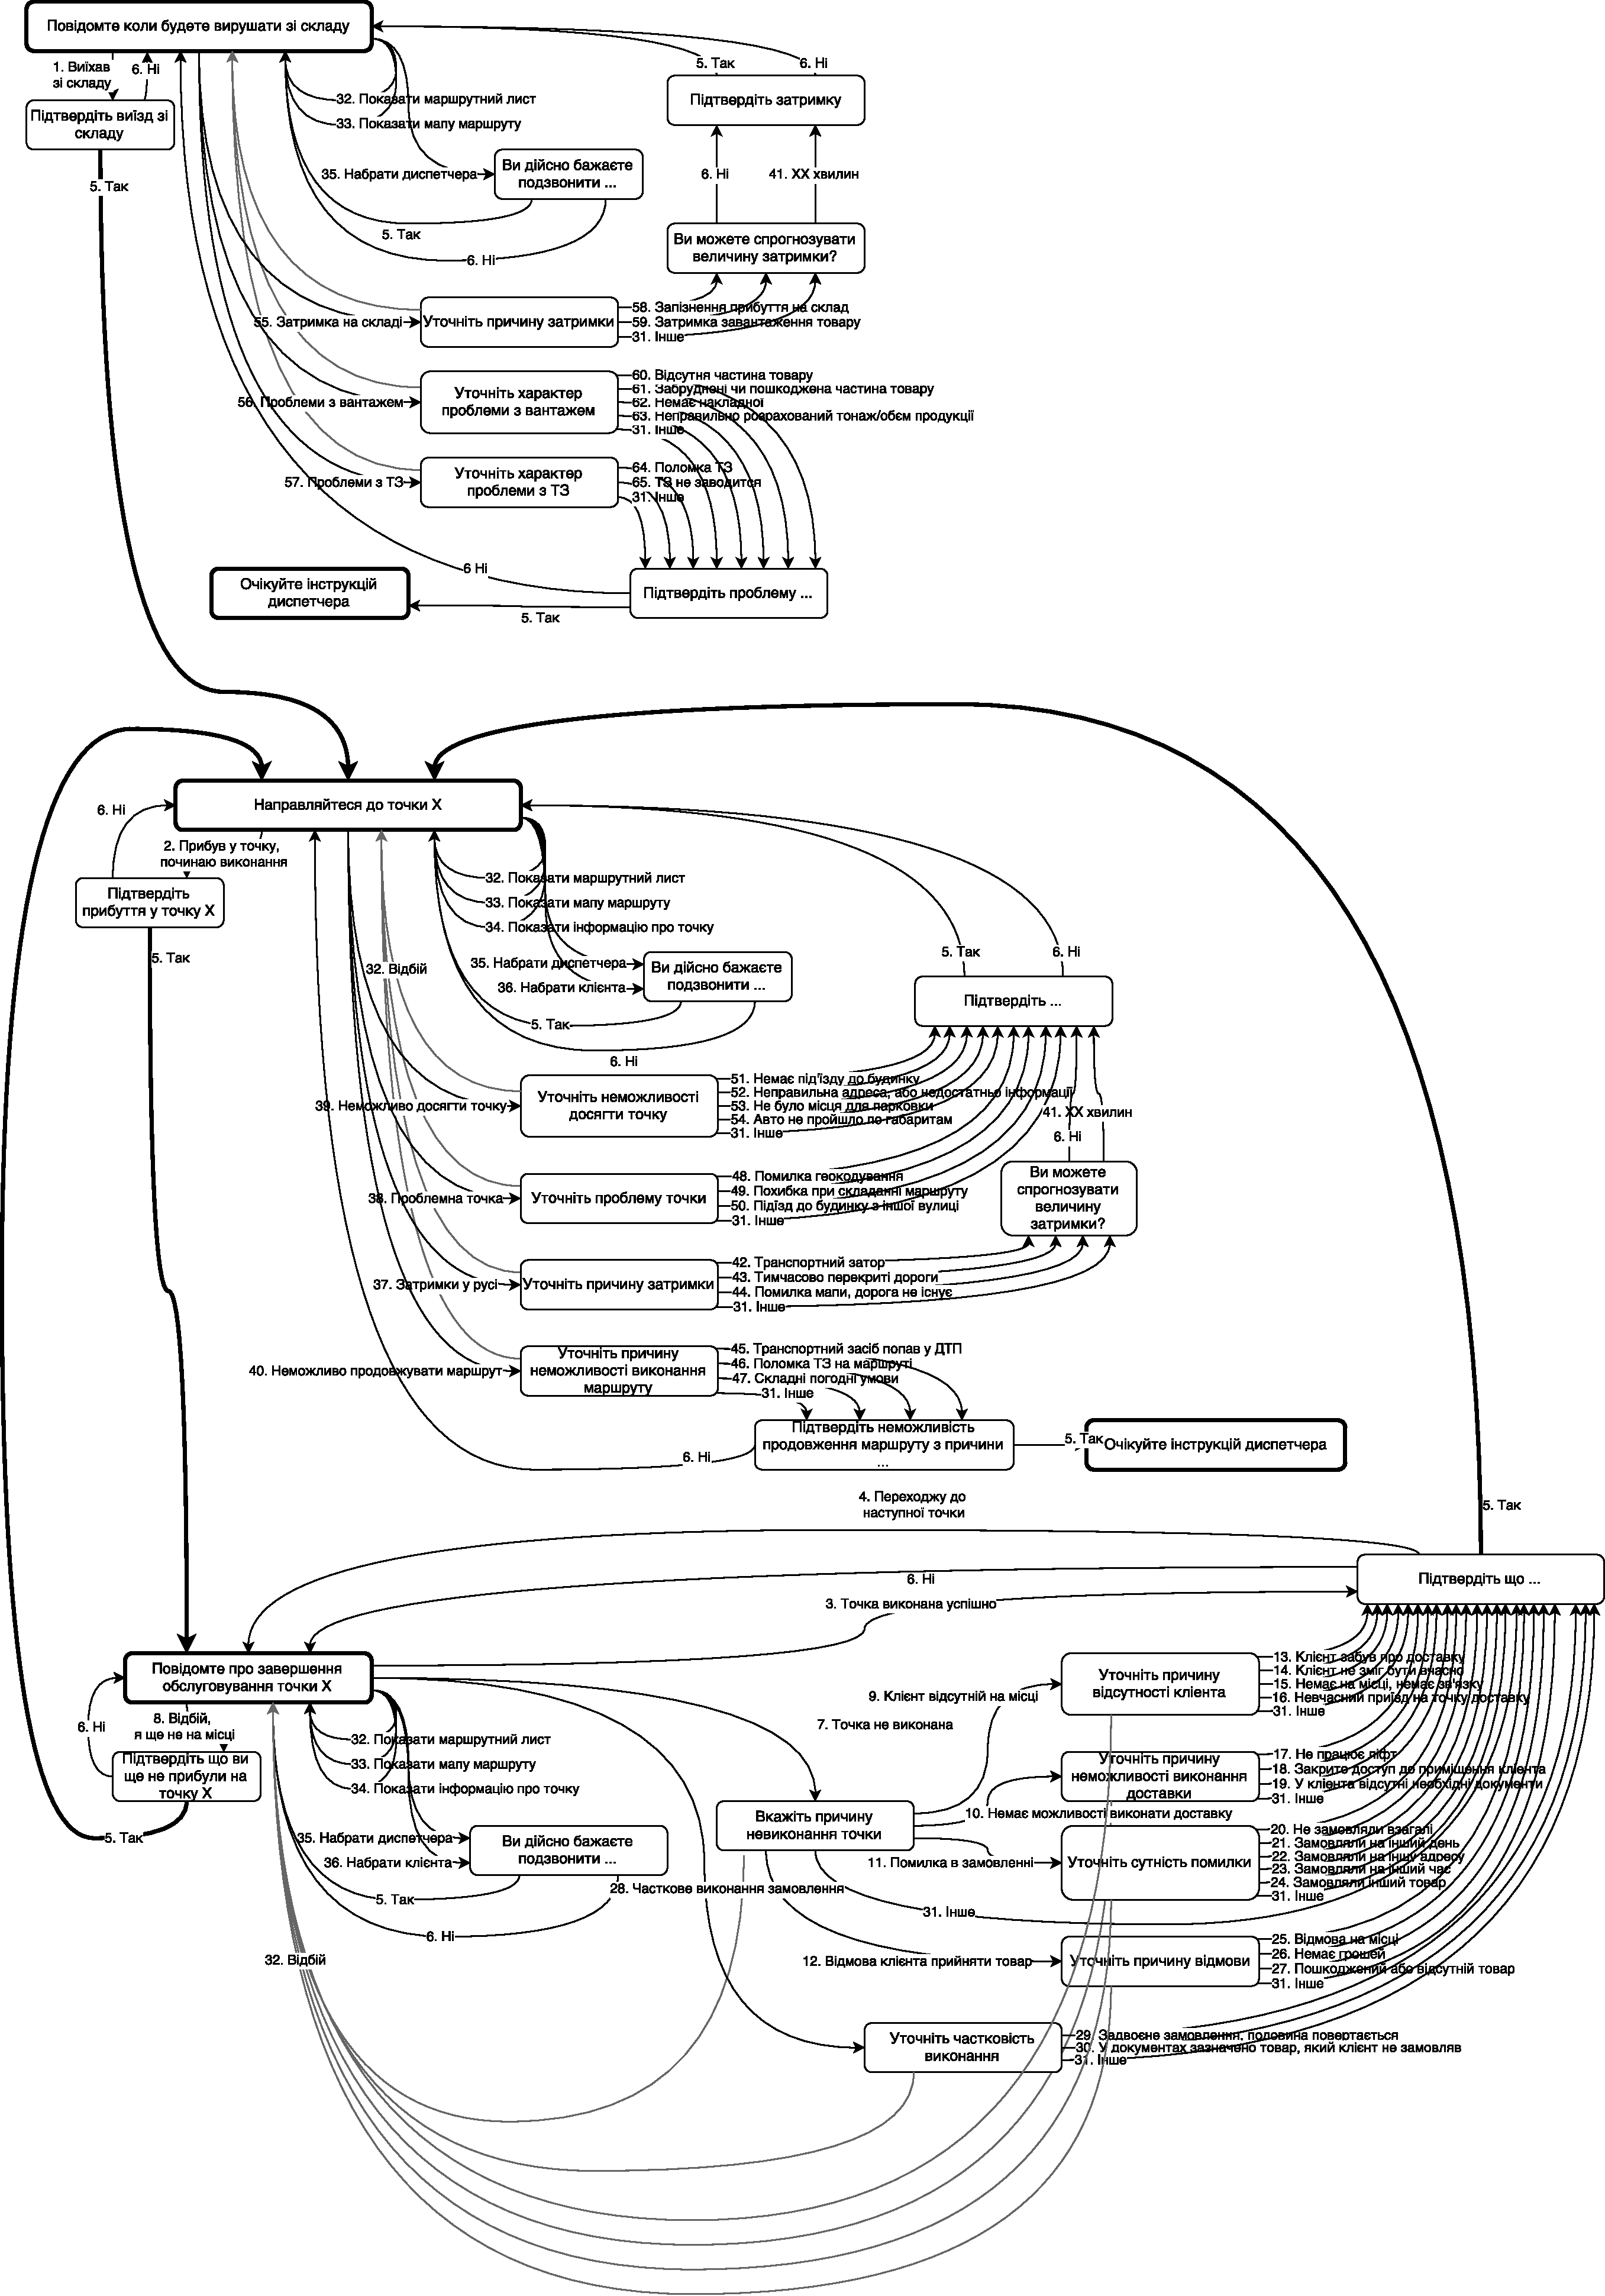
\includegraphics [width=1\linewidth] {13_complete_scenario_graph}
	\caption{Повне дерево сценаріїв голосової взаємодії}
	\label{img:13_complete_scenario_graph}
\end{figure}

В повному дереві сценаріїв усіх етапів дистрибуції (рис. \ref{img:13_complete_scenario_graph}) враховані всі можливі причини затримки або невиконання етапів «склад», «дорога», «точка доставки», а для таких випадків при неможливості виконання етапу існує вказівка (інструкції) диспетчера щодо подальших дій водія.

З приведеного дерева сценарії були виділені та пронумеровані унікальні контексти на основі можливих реплік які повинні бути розпізнані в кожному з контекстів. Ці дані приведені у таблиці \ref{tbl:context_reactions}

\begin{table} [!htb]%
	\caption{Перелік контекстів та можливих реакцій у них}%
	\label{tbl:context_reactions}% label всегда желательно идти после caption
%	\renewcommand{\arraystretch}{1.6}%% Увеличение расстояния между рядами, для улучшения восприятия.
	\def\tabularxcolumn#1{m{#1}}
	\centering
	\begin{tabularx}{0.7\textwidth}{@{}>{\centering}m{3.0cm} | >{\raggedright\arraybackslash}X@{}}% Вертикальные полосы не используются принципиально, как и лишние горизонтальные (допускается по ГОСТ 2.105 пункт 4.4.5) % @{} позволяет прижиматься к краям
		\toprule     %%% верхняя линейка
		№ Контексту & Можливі реакції	\\
		\midrule %%% тонкий разделитель. Отделяет названия столбцов. Обязателен по ГОСТ 2.105 пункт 4.4.5 
		1 & 5, 6 \\
		2 & 6, 41 \\
		3 & 1, 32, 33, 35, 55, 56, 57 \\
		4 & 8, 31, 58, 59 \\
		5 & 8, 31, 60, 61, 62, 63 \\
		6 & 8, 31, 64, 65 \\
		7 & 2, 32, 33, 34, 35, 36, 37, 38, 39, 40 \\
		8 & 8, 31, 51, 52, 53, 54 \\
		9 & 8, 31, 48, 49, 50 \\
		10 & 8, 31, 42, 43, 44  \\
		11 & 8, 31, 45, 46, 47 \\
		12 & 3, 7, 8, 28, 32, 33, 34, 35, 36 \\
		13 & 4, 5, 6 \\
		14 & 8, 9, 10, 11, 12, 31 \\
		15 & 8, 13, 14, 15, 16, 31 \\
		16 & 8, 17, 18, 19, 31 \\
		17 & 8, 20, 21, 22, 23, 24, 31 \\
		18 & 8, 25, 26, 27, 31 \\
		19 & 8, 29, 30, 31 \\
		\bottomrule %%% нижняя линейка
	\end{tabularx}%
\end{table}

Як показано на схемі структури (рис. \ref{img:rsgu_struct}) системи формалізації голосової інформації складається з двох основних модулів: Фонемного стенографа для перетворення звукового сигналу у текстову пофонемну репрезентацію, та ядра рефлекторної системи голосового управління (РГСУ) яке класифікує текстову пофонемну репрезентацію згідно до заданого набору можливих команд.

В якості модуля фонемного стенографа Української мови використовується попередня розробка \cite{Pylypenko_2008}, виконана у вигляді бінарного додатку, набору бібліотек і конфігураційних файлів для платформи Windows.

У якості ядра РГСУ може бути використана інтелектуальна рефлекторна система на основі теорії несилової взаємодії. Для цього фонеми кожної репліки були розбиті на послідовні набори фонем різної довжини, відомі в методах обробки тексту як N-грами. Для застосування формул приведених вище потрібно було визначити безумовну ймовірність вибору для кожної реакції та умовну ймовірність вибору кожної реакції за наявності впливу від кожного N-граму. Ці значення були розраховані статистично на основі аналізу тестового набору даних. Далі на основі формул приведених вище, через інформованість та визначеність була розрахована сумісна умовна ймовірність реакції при існуванні впливів від всіх N-грамів у репліці.

Розробка ядра РГСУ була виконана на мові JavaScript у середовищі node.js з використанням бази даних SQLite. Відкритий вихідний код розробленої системи є у публічному доступі \cite{code1}.

\subsection{Використання методу згорткових нейронних мереж для класифікації фонемної репрезентації голосових команд}

Для перевірки роботи інтелектуальних рефлекторних систем було використано модель на основі згорткових нейронних мереж (ЗНМ). Модель на основі ЗНМ є альтернативною реалізацією ядра РГСУ зі схеми на рис. \ref{img:rsgu_struct}.

ЗНМ для роботи з фонемами найбільше нагадує ЗНМ в задачі класифікації текстів \cite{Kim_2014}, але оперує з «текстом» не по словах, а пофонемно, що схоже на роботу з текстом посимвольно \cite{Zhang_2016}.

Система виконана на мові Python з використанням фреймворку TensorFlow на основі реалізації ЗНМ для роботи з текстом \cite{Britz_2015}. Відкритий вихідний код розробленої системи є у публічному доступі \cite{code2}.

Структура нейронної мережі може бути представлена наступним чином.

Фонеми представлені у вигляді one-hot векторів. Фрази нормалізовані за максимальною довжиною, з використанням вектора з усіма нулями в якості заповнювача.

На відміну від роботи по словам, вкладений шар (embedding layer) відсутній, оскільки потужність множини фонем набагато нижчий ніж потужність множини слів, і такий шар не є необхідним. З іншого боку, деякі фонеми схожі на інші, а деякі ні, тому використання вкладень може бути доцільним для передачі цієї схожості, а не тільки для зниження розмірності. Навчання вкладеного шару потребує великого об’єму вхідних даних, тому в даній роботі не буде розглянуто.

Використовується комбінований згортковий шар (convolution layer), який складається з декількох паралельних одновимірних шарів з різними варіантами кроку фільтра.

Для агрегації кожного зі згорткових шарів використовується агрегаційний шар (pooling layer) з вибором одного максимального значення (1-max-pooling).

Виходи агрегаційних підшарів різного розміру кроку згортки комбінується в один вектор значень.

У якості повнозв’язного шару використовується класичний перцептрон, який може мати активаційну функцію у вигляді неспадних диференційованих функцій, що діють на множині дійсних чисел. У нашому випадку для функції активації використаємо ReLU.

Традиційно для задач класифікації в якості функції втрат використовується кросс-ентропія. Інакше кажучи, робимо мінімізацію різниці між виходом нейронної мережі і відповідним набором фонем. Різницею, якраз і буде величина кросс-ентропії.

Для навчання використовується Adam-алгоритм зворотного розповсюдження помилки із стохастичним градієнтним спуском, який дозволяє регулювати величину швидкості навчання в залежності від параметрів з виконанням більших оновлень для 32-х або 16-ти рідких параметрів і маленьких оновлень для більш частих параметрів \cite{art4}.

\begin{table} [!hb]%
	\caption{Відсоток розпізнавання ІРС та ЗНМ}%
	\label{tbl:data_total}% label всегда желательно идти после caption
%	\renewcommand{\arraystretch}{1.4}%% Увеличение расстояния между рядами, для улучшения восприятия.
	\def\tabularxcolumn#1{m{#1}}
	\begin{tabularx}{\textwidth}{@{}>{\centering}X | >{\centering}X >{\centering}X | >{\centering}X >{\centering}X | >{\centering\arraybackslash}X@{}}% Вертикальные полосы не используются принципиально, как и лишние горизонтальные (допускается по ГОСТ 2.105 пункт 4.4.5) % @{} позволяет прижиматься к краям
		\toprule     %%% верхняя линейка
		№ Контексту & Точність розпізнавання ЗНМ & Кількість розпізнаних стимулів ЗНМ & Точність розпізнавання ІРС & Кількість розпізнаних стимулів ІРС & Загальна кількість стимулів в контексті	\\
		\midrule %%% тонкий разделитель. Отделяет названия столбцов. Обязателен по ГОСТ 2.105 пункт 4.4.5 
		1 & 92.0 & 92 & 85 & 85 & 100 \\
		3 & 99.4 & 348 & 86.6 & 303 & 350 \\
		4 & 99.0 & 198 & 87 & 174 & 200 \\
		5 & 98.0 & 294 & 83 & 249 & 300 \\
		6 & 97.5 & 195 & 83.5 & 167 & 200 \\
		7 & 95.6 & 478 & 77.4 & 387 & 500 \\
		8 & 98.7 & 296 & 85.7 & 257 & 300 \\
		9 & 97.2 & 243 & 88.8 & 221 & 250 \\
		10 & 96.4 & 241 & 86.4 & 216 & 250 \\
		11 & 96.4 & 241 & 82.4 & 206 & 250 \\
		12 & 95.1 & 428 & 75.1 & 338 & 450 \\
		13 & 94.0 & 141 & 84.1 & 122 & 150 \\
		14 & 95.0 & 285 & 73 & 219 & 300 \\
		15 & 92.0 & 276 & 78 & 234 & 300 \\
		16 & 96.8 & 242 & 84 & 210 & 250 \\
		17 & 95.1 & 333 & 64.6 & 226 & 350 \\
		18 & 93.6 & 234 & 74 & 185 & 250 \\
		19 & 98.0 & 196 & 82.5 & 165 & 200 \\
		По всій вибірці & 90.2 & 2885 & 63.7 & 2038 & 3200 \\	
		\bottomrule %%% нижняя линейка
	\end{tabularx}%
\end{table}

Результати моделювання обома описаними методами наведені у таблиці \ref{tbl:data_total}. Розміри N-грам при моделюванні інтелектуальними рефлекторними системами були вибрані в діапазоні 2--4. Розміри згорткових фільтрів при моделюванні згортковими нейронними мережами також були взяті в діапазоні 2--4.

\section{Обговорення результатів моделювання різними методами та перспективи подальшого дослідження}

Для експериментальної перевірки ефективності розроблених методів були зібрані голосові дані 23 різних дикторів (11 жінок, 12 чоловіків), які надиктували 64 реакції наявні в дереві сценаріїв (рис. \ref{img:13_complete_scenario_graph}) використовуючи різні варіанти формулювання команд. Всього було зібрано 3200 голосових зразків команд. Дані оброблені фонемним стенографом є у відкритому доступі разом з вихідним кодом моделей \cite{code1,code2}.

Дані були розділені на тренувальну та тестову вибірки методом кросс-валідації використовуючи 5 груп. Тобто дані були розділені на 5 груп випадковим чином і моделювання було проведене 5 разів, використовуючи кожну з 5 груп як тестову вибірку і 4 інших як тренувальну. Такий підхід дозволяє краще оцінити точність методу, оскільки кожен з зразків даних бере участь у оцінці.

Як можна бачити з таблиці \ref{tbl:data_total}, згорткові нейронні мережі показали кращий результат класифікації набору фонем на команди. 

Також ми бачимо, що найменший відсоток розпізнавання при використанні обох методів у випадку коли контексти не використовуються і моделювання відбувається одночасно всіх команд. З цього можна зробити висновок що використання дерева сценаріїв та контекстів є доцільним.

Також при проведенні досліджень було відмічено, що навчання при використанні методу ІРС набагато швидше ніж ЗГМ, але фактичне розпізнавання на навченій системі відбувається швидше з використанням згорткових нейронних мереж.

Якщо детально розглянути ядро розрахунків ІРС то видно що воно дуже нагадує повнозв'язний шар нейронної мережі. Умовна ймовірність вибору реакції $A_i$, при існуванні впливу $B_j$ ($p(A_i/B_j)$) відповідає вагам шару нейронної мережі ($W = |w_ij|$), а безумовна ймовірність вибору реакції $A_i$ ($p(A_i)$) відповідає зміщенням ($B = |b_i|$). На відміну від класичного перцептрону, в якому функція активації застосовується до результата добутку матриць ($Y=f(WX + B)$), функція активації в РГСУ набагато складніша, до того ж працює із вагами та зміщеннями напряму, як наприклад радіально-базисна функція активації.

В методом інтелектуальних рефлекторних систем параметри $p(A_i/B_j)$ та $p(A_i)$ розраховуються частотно. Фактично при використанні цього методу не має етапу навчання аналогічного до такого при навчанні нейронних мереж. Такий підхід більше схожий на метод найменших квадратів, де параметри можуть бути напряму вирахувані і не потребують оптимізації.
Але якщо обмежити діапазон можливих значень параметрів інтервалом $[0, 1]$ який відповідає можливим значенням ймовірності, то можна спробувати отримати оптимальні значення цих параметрів шляхом навчання методом зворотного розповсюдження помилки.

Попередня обробка фонем (об'єднання послідовних наборів фонем різної довжини) відповідає згортковим та агрегаційним шарам згорткової нейронної мережі, але замість підбору найкращих фільтрів, використовується фіксований набір. Він включає в себе всі можливі комбінації фонем (N-грами) відповідно до розміру вікна фільтру. Такий фіксований набір фільтрів одночасно є набагато більшим за необхідний для ефективного розпізнавання і при цьому не достатньо повним, оскільки не включає нелінійні комбінації та пропуски, коли деякі фонеми у вікні фільтра важливіші. Тому навчання оптимальних параметрів фільтру в нейронній мережі може дати кращий результат.

Функція активації РГСУ достатньо складна, і її розрахунок набагато довший ніж ReLU чи інші функції активації  повнозв'язних шарів. Оскільки в класичному підході РГСУ немає ітеративного навчання, це не є критичною проблемою. Але саме порівняння інтроформаційної функції активації з класичними функціями нелінійності нейронних мереж в рівних умовах, може дати незалежну оцінку її ефективності.


\section{Висновки}

Аналіз практики управління дистрибуцією показав що при впровадженні систем оптимізації маршрутів транспортних засобів залишається не забезпеченою необхідність спрощення комунікації з диспетчером для коригування маршрутів після виникнення позапланових ситуацій. Основним недоліком програм фіксації позапланових ситуацій на пристроях з сенсорним управлінням є затримка та відволікання водія від основної функції керування транспортним засобом, що в більшості випадків призводить до уникнення водіями коригування маршрутів і виконання доставки повністю поза планом. Основним недоліком сучасних систем розпізнавання голосу є необхідність постійного доступу до мережі інтернет, а ті засоби які можуть бути встановлені на телефон не мають достатньої якості розпізнавання мови.

У роботі запропоновано модель формалізації голосової інформації в системах диспетчерського контролю за рухом автотранспорту, з використанням дерева сценаріїв для моделювання голосової взаємодії між водієм та системою підтримки диспетчеризації автотранспорту, та інтелектуальної рефлекторної системи голосового управління для класифікації голосових команд описаних у дереві сценаріїв.

Розроблено контекстну модель голосової взаємодії водія в системах диспетчерського контролю за рухом автотранспорту у вигляді дерева сценаріїв що дозволяє виділити контексти розпізнавання голосових команд, за рахунок чого скоротити різноманіття команд і покращити якість розпізнавання. У результаті аналізу зібраних статистичних даних, зауважень та коментарів щодо процесу доставки різних вантажів автомобільним транспортом у провідних логістичних компаніях, було запропоновано повне дерево сценаріїв усіх етапів дистрибуції «склад – дорога – точка доставки» з вказівкою контекстів і з включенням можливих реакцій в них.

Метод інтелектуальних рефлекторних систем голосового управління набув подальшого розвитку. Запропоновано використовувати інші методи класифікації наборів фонем у команди у якості ядерного компонента системи. Було розроблено альтернативний класифікатор команд з використанням методу згорткових нейронних мереж.

Проведене моделювання рефлекторної системи голосового управління у системах диспетчерського контролю за рухом автотранспорту на основі зібраних голосових даних 23 різних дикторів (11 жінок, 12 чоловіків), які надиктували 64 реакції наявні в дереві сценаріїв використовуючи різні варіанти формулювання команд. Моделювання було проведено з використанням двох альтернативних класифікаторів команд у якості ядерного компоненту РГСУ: з використанням методу інтелектуальних рефлекторних систем та згорткових нейронних мереж.

Аналіз результатів моделювання показав що застосування дерева сценаріїв та розбиття повного набору команд на контексти є доцільним, оскільки значення точності без використання контекстів є найменшими для обох методів класифікації. Порівняння результатів моделювання для різних методів класифікації показало що обидва методи можуть бути використані на практиці, причому навчання моделі при використанні методу інтелектуальних рефлекторних систем набагато швидше ніж для згорткових нейронних мереж, але фактичне розпізнавання на навченій системі відбувається швидше з використанням згорткових нейронних мереж. Точність моделювання також вища при використанні згорткових нейронних мереж.

Було визначено спільні риси методів згорткових нейронних мереж та інтелектуальних рефлекторних систем та окреслено перспективи подальшого дослідження їх порівняння в більш незалежних умовах.

У результаті проведеного дослідження було розроблено та налаштовано інтелектуальну рефлекторну систем голосового управління готову до впровадження, яка дозволить підвищити ефективність та зручності роботи водіїв в системах дистрибуції та дасть змогу автоматизувати процеси управління дистрибуцією на етапі «останньої милі», покращуючи рівень сервісу та знижуючи витрати.